
% listing (file)

\lstinputlisting[%
language={},%
caption={[short.]description sentence.},%
label={lst:traingen-help}]%
{listings/traingen-help.txt}

% listing

\begin{lstlisting}[%
language={},%
caption={[short.]description sentence.},%
label={lst:traingen-help}]
code
\end{lstlisting}

% figure (htp = here, top, bottom)

\begin{figure}[htb]
  \centering
  \includegraphics[width=8cm]{filenameWithoutExtension}
  \caption[Short description for list of figures.]{%
  The long description text.
  }\label{fig:}
\end{figure}

% figure with subfigures
\begin{figure}[htb]
  \centering
  \begin{subfigure}[t]{0.35\linewidth}
    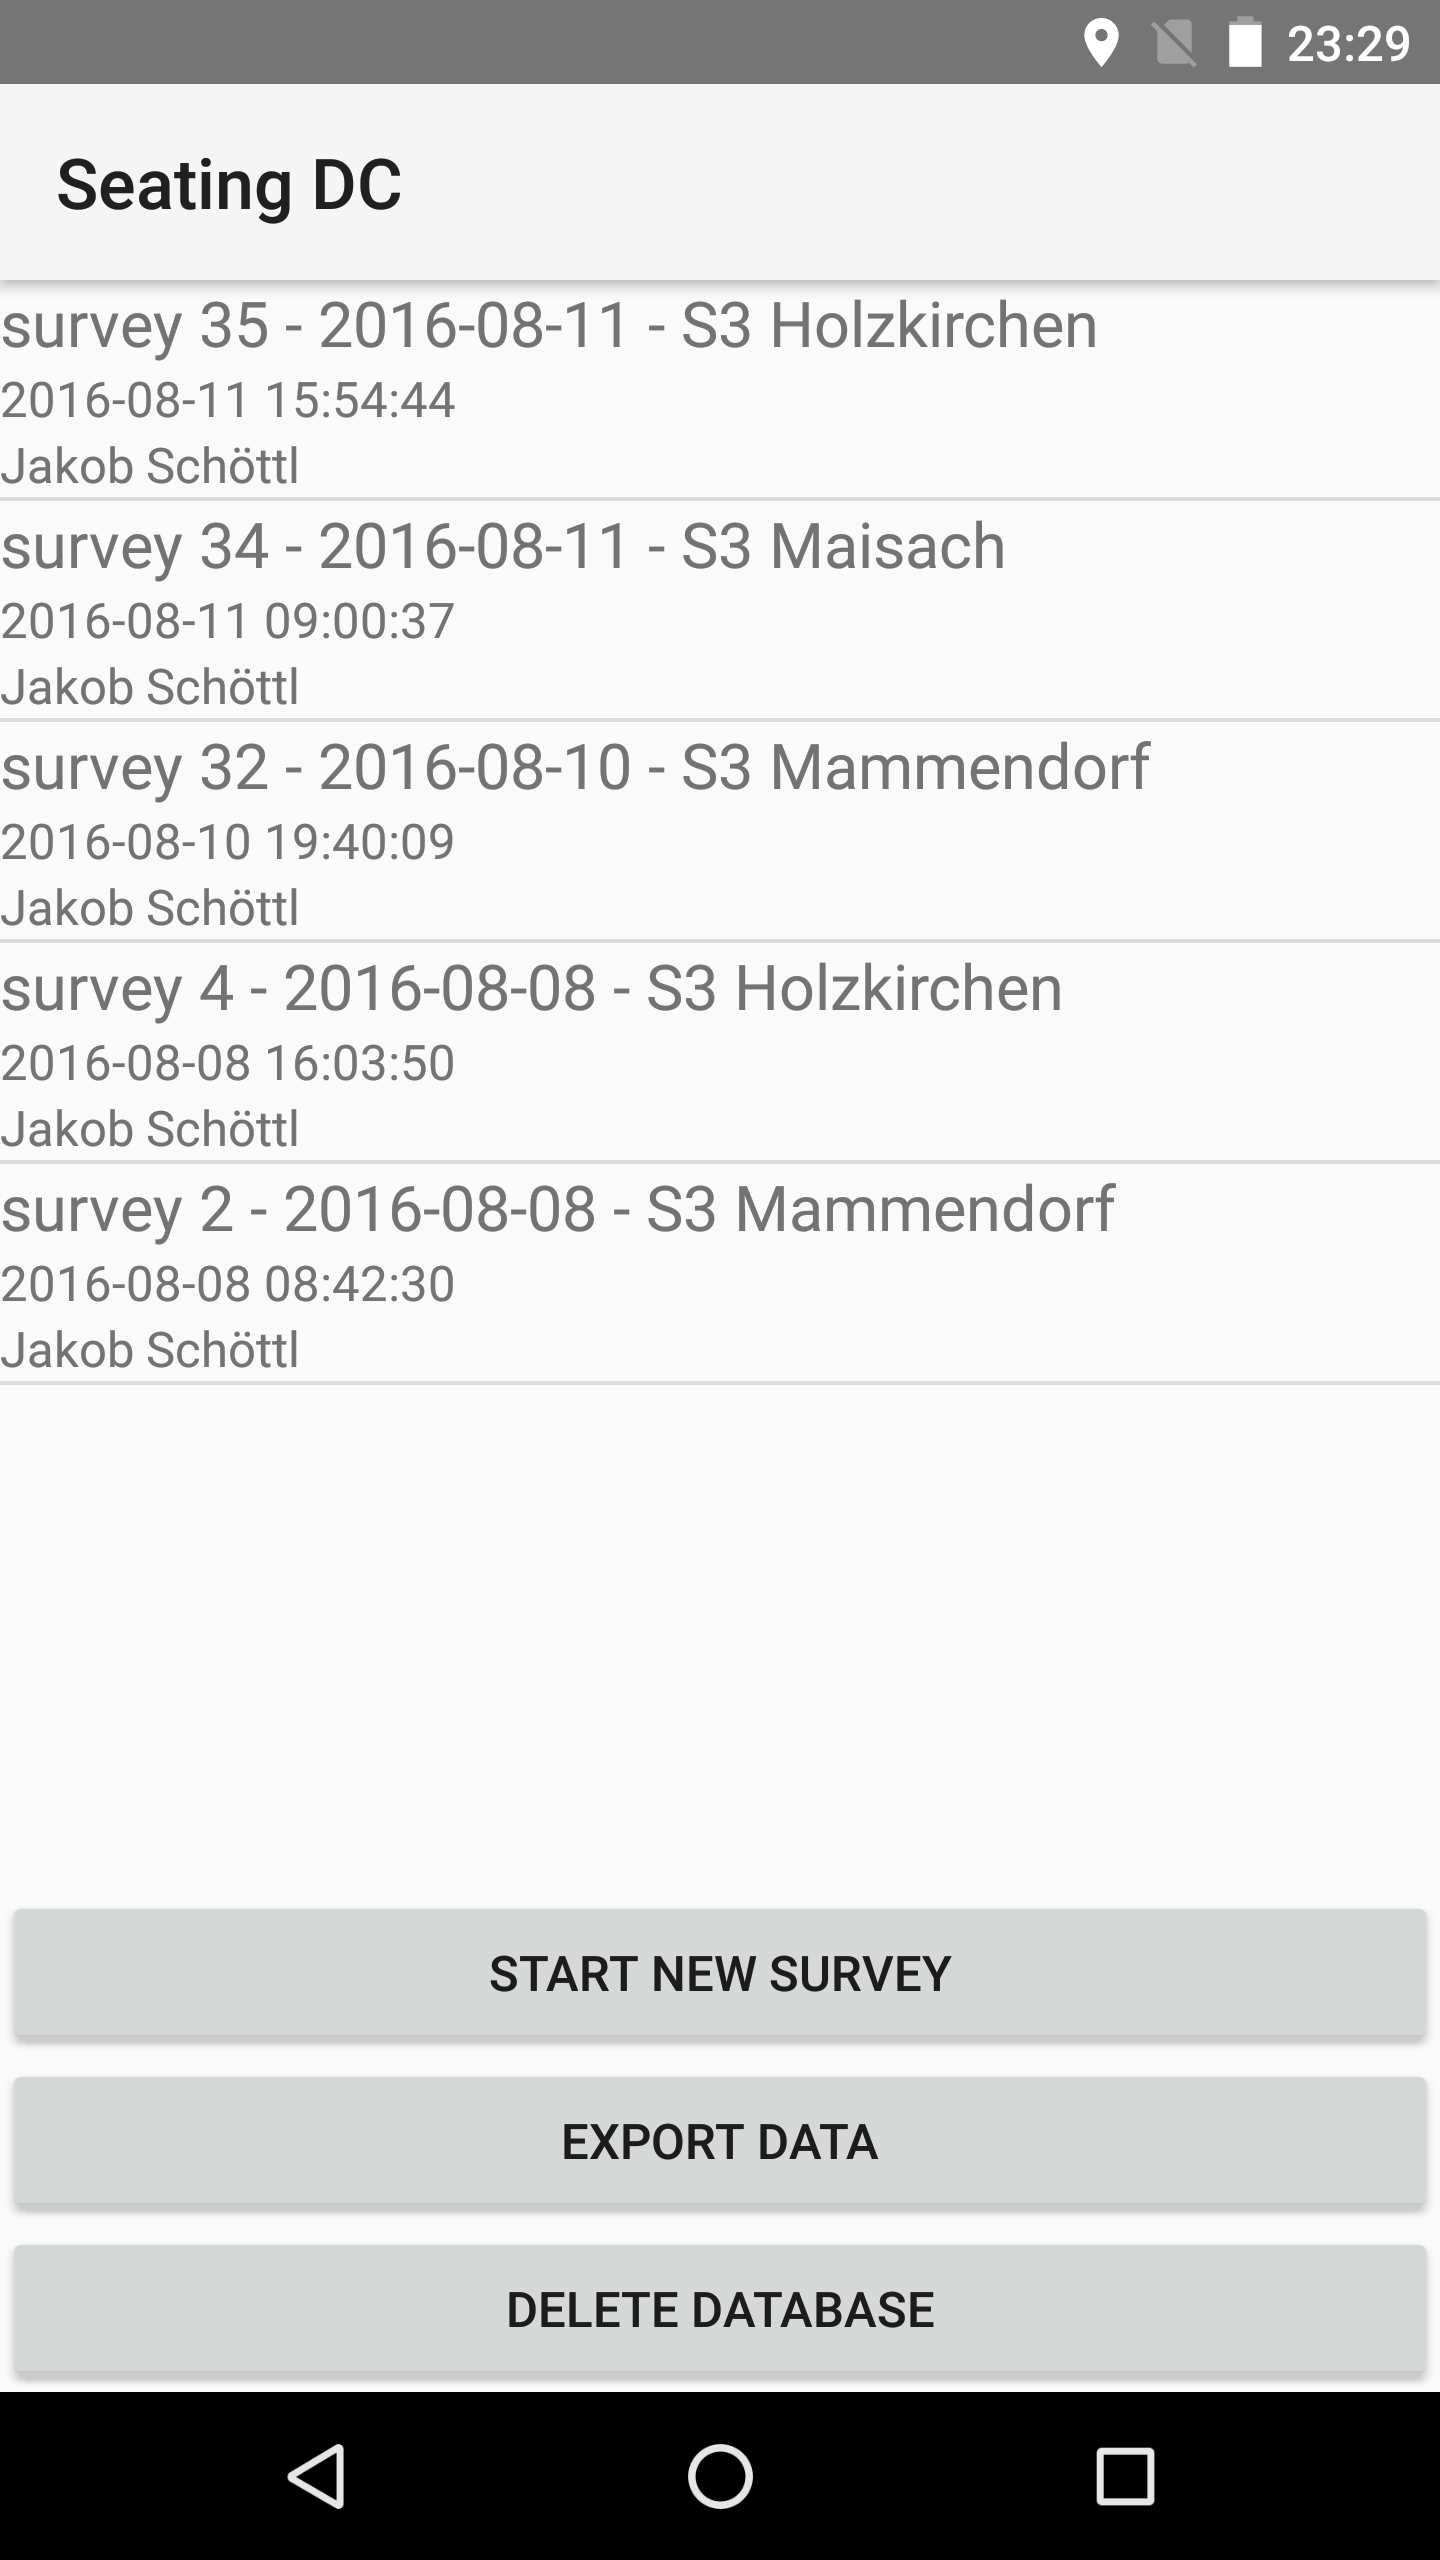
\includegraphics[width=\linewidth]{screenshot-app-1.png}
    \caption{Start screen}
    \label{fig:app-screen-1}
  \end{subfigure}
  \hspace{0.6cm}
  \begin{subfigure}[t]{0.35\linewidth}
    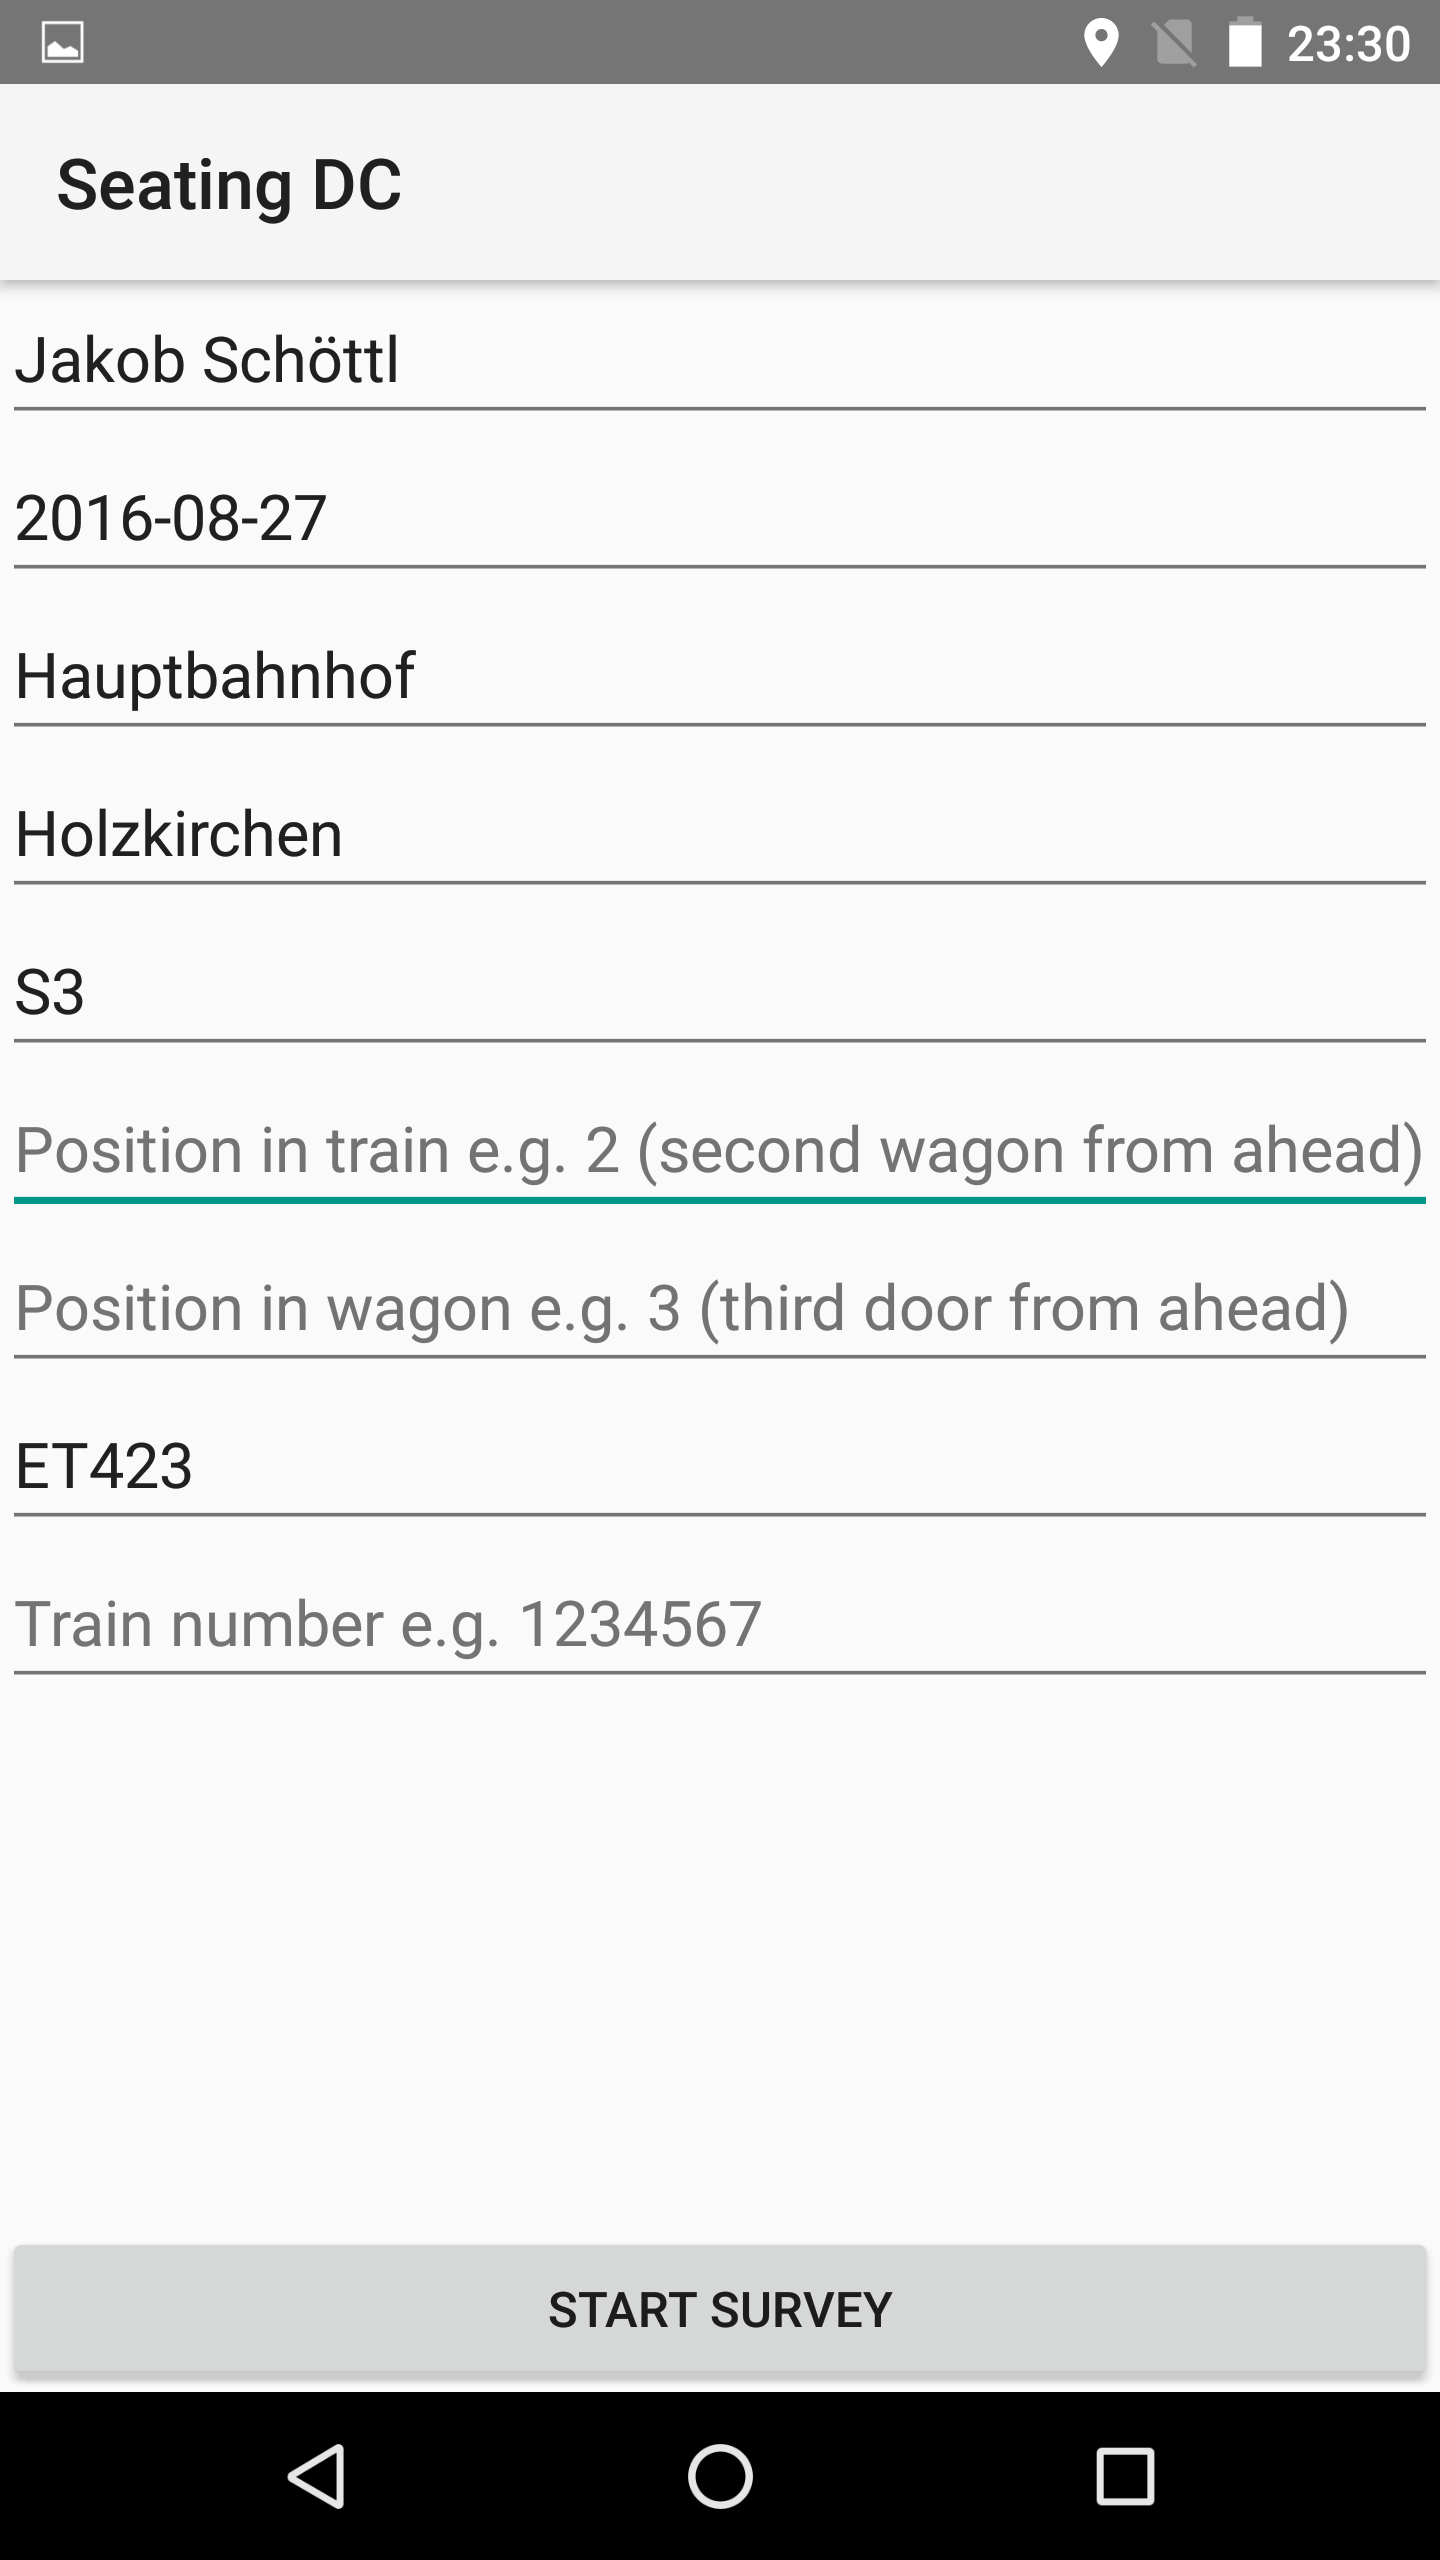
\includegraphics[width=\linewidth]{screenshot-app-2.png}
    \caption{Survey meta data}
    \label{fig:app-screen-2}
  \end{subfigure}
  \\
  \vspace{0.6cm}
  \begin{subfigure}[t]{0.35\linewidth}
    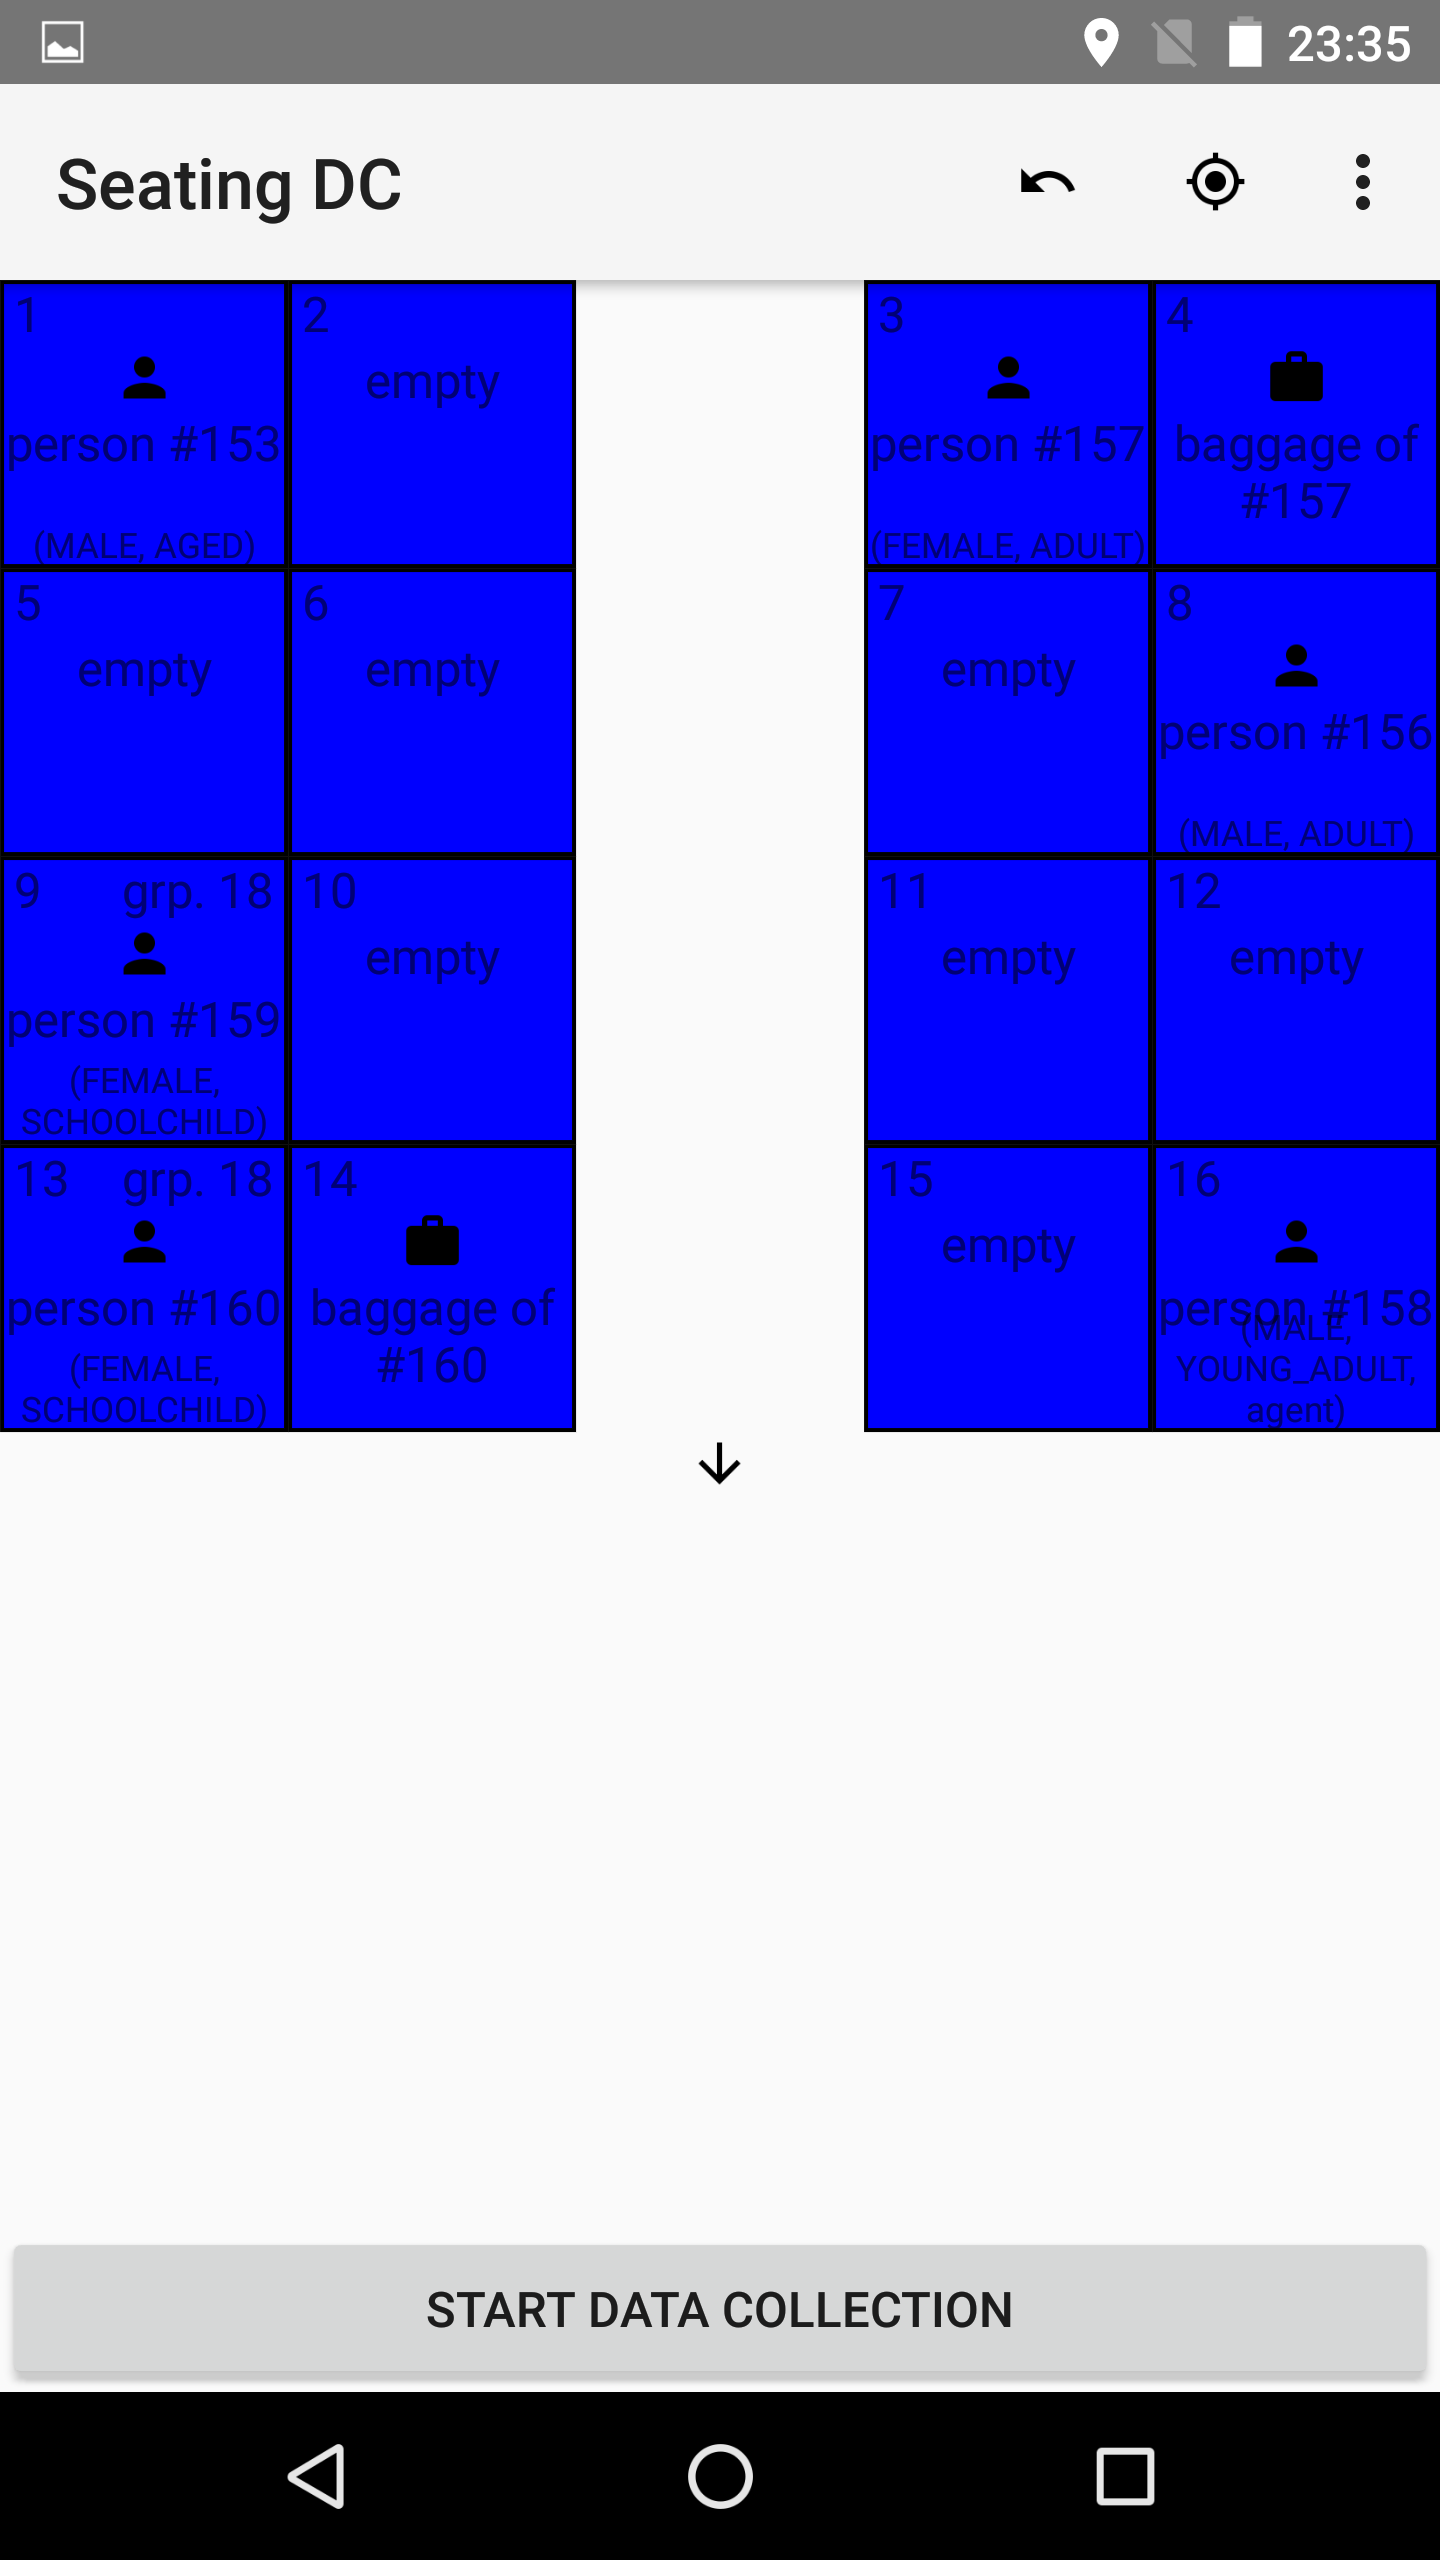
\includegraphics[width=\linewidth]{screenshot-app-3.png}
    \caption{Initialization phase}
    \label{fig:app-screen-3}
  \end{subfigure}
  \hspace{0.6cm}
  \begin{subfigure}[t]{0.35\linewidth}
    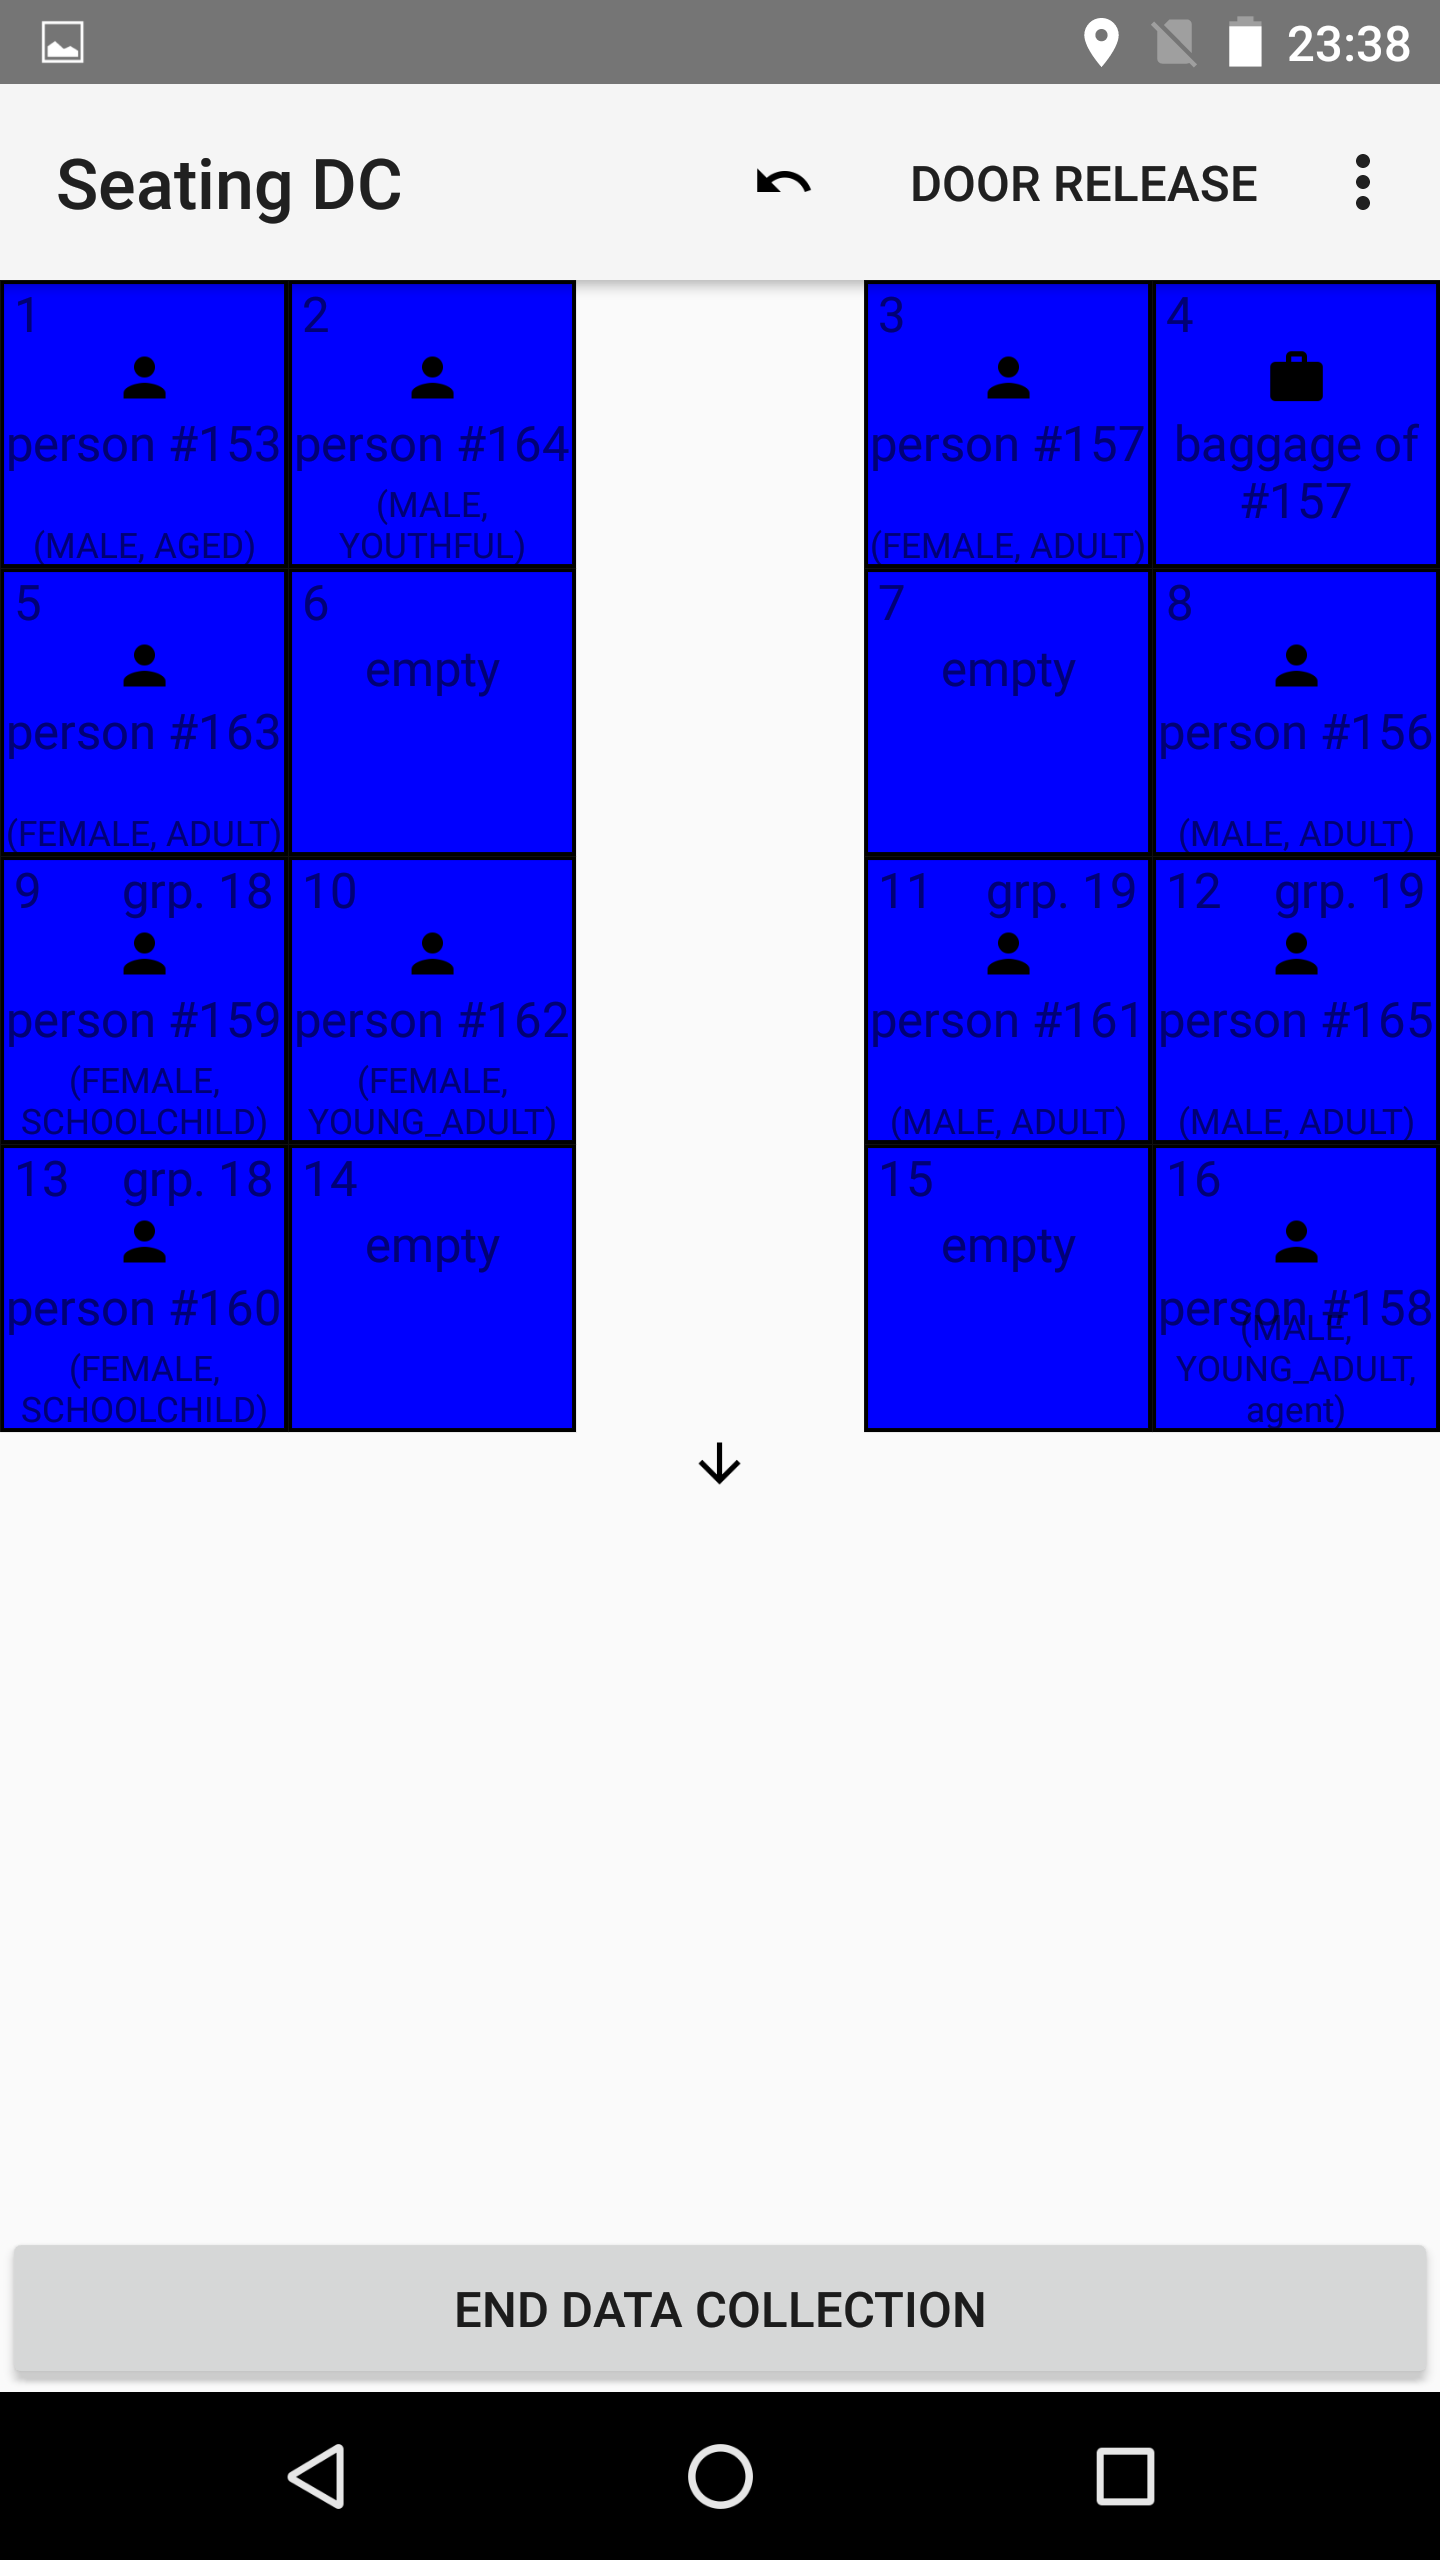
\includegraphics[width=\linewidth]{screenshot-app-4.png}
    \caption{Real-time data collection}
    \label{fig:app-screen-4}
  \end{subfigure}
  \caption[short]{%
  Screens of the data collection app on a Nexus~6 smartphone.
  }\label{fig:app-screens}
\end{figure}


% table

% :Tab /&
% :Tab /\\\\

\begin{table}[h]
\begin{tabular}{l|l}
  Target Platform           & Android              \\
  Target \acs{SDK} version  & 23                   \\
  Minimum \acs{SDK} version & 21                   \\
  Development platform      & Arch Linux           \\
  Development \acs{IDE}     & Android Studio 2.1.2 \\
  Development device        & Motorola Nexus~6     \\
\end{tabular}
  \caption[Short description]{%
  Table of technical details on the app development.
  }\label{tab:app-dev}
\end{table}


% small enumeration

\begin{itemize}[noitemsep,nolistsep]
\end{itemize}
